\autobookmark
\begin{frame}[t]{ASE can be modeled as multidimensional integral}
  \begin{columns}[T]
    \begin{column}{.5\textwidth}
      \myonly{1}{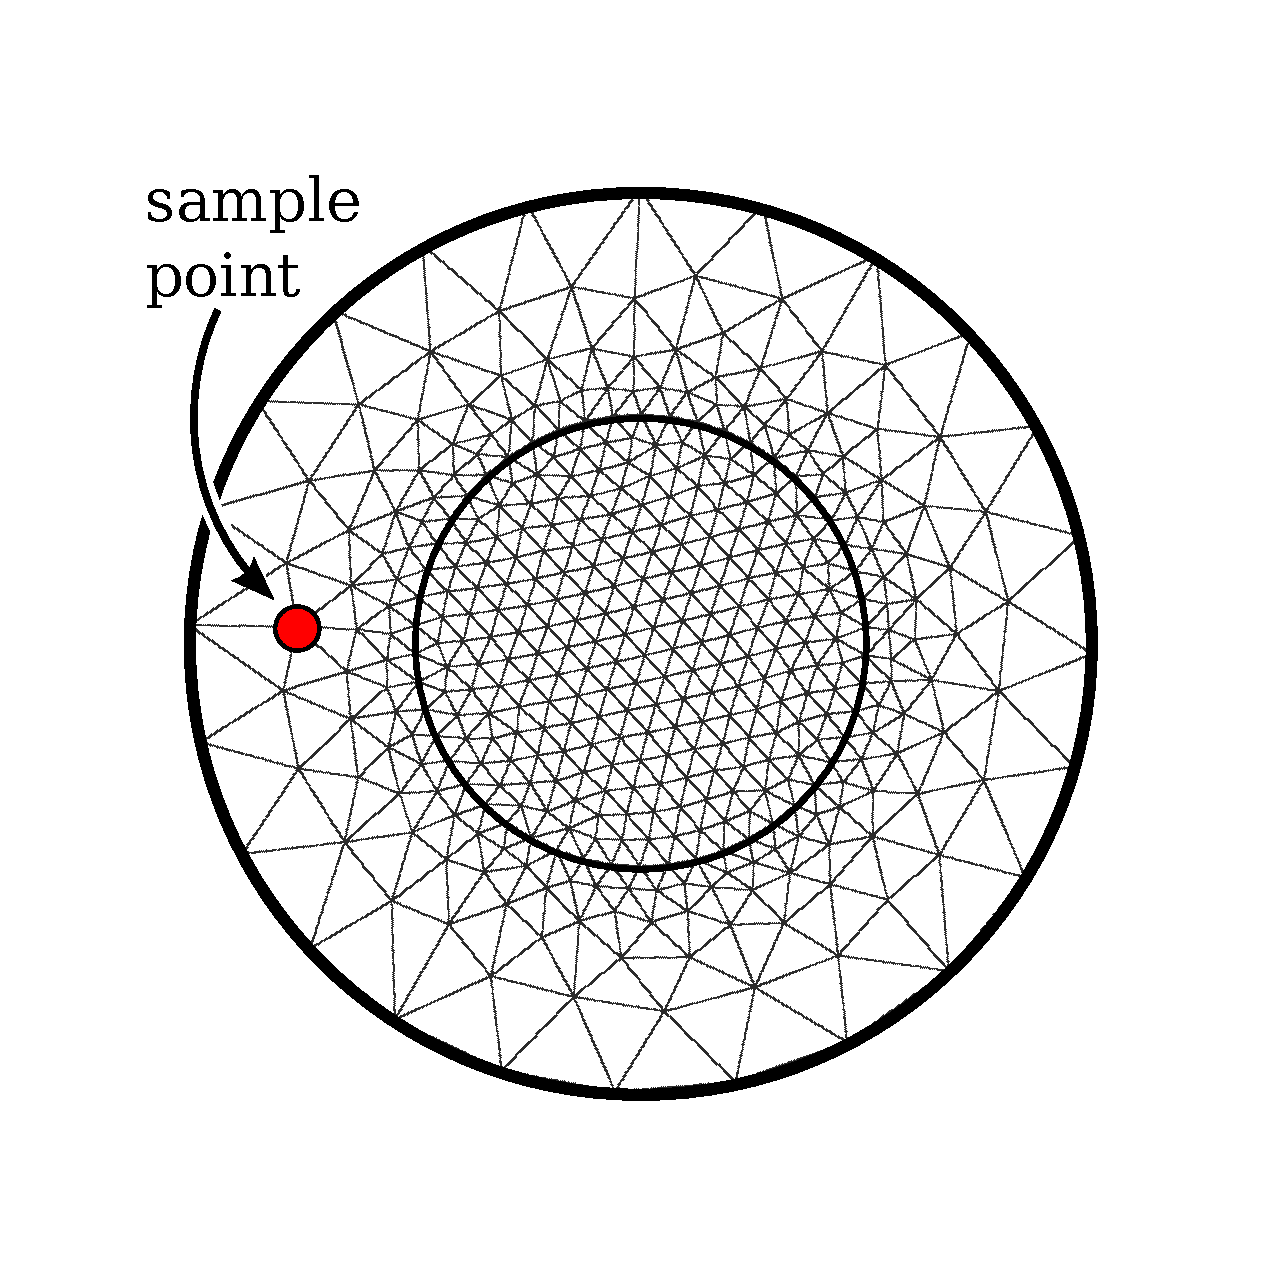
\includegraphics[height=0.55\paperheight]{graphics/monte_carlo_description_0.pdf}}
      \myonly{2}{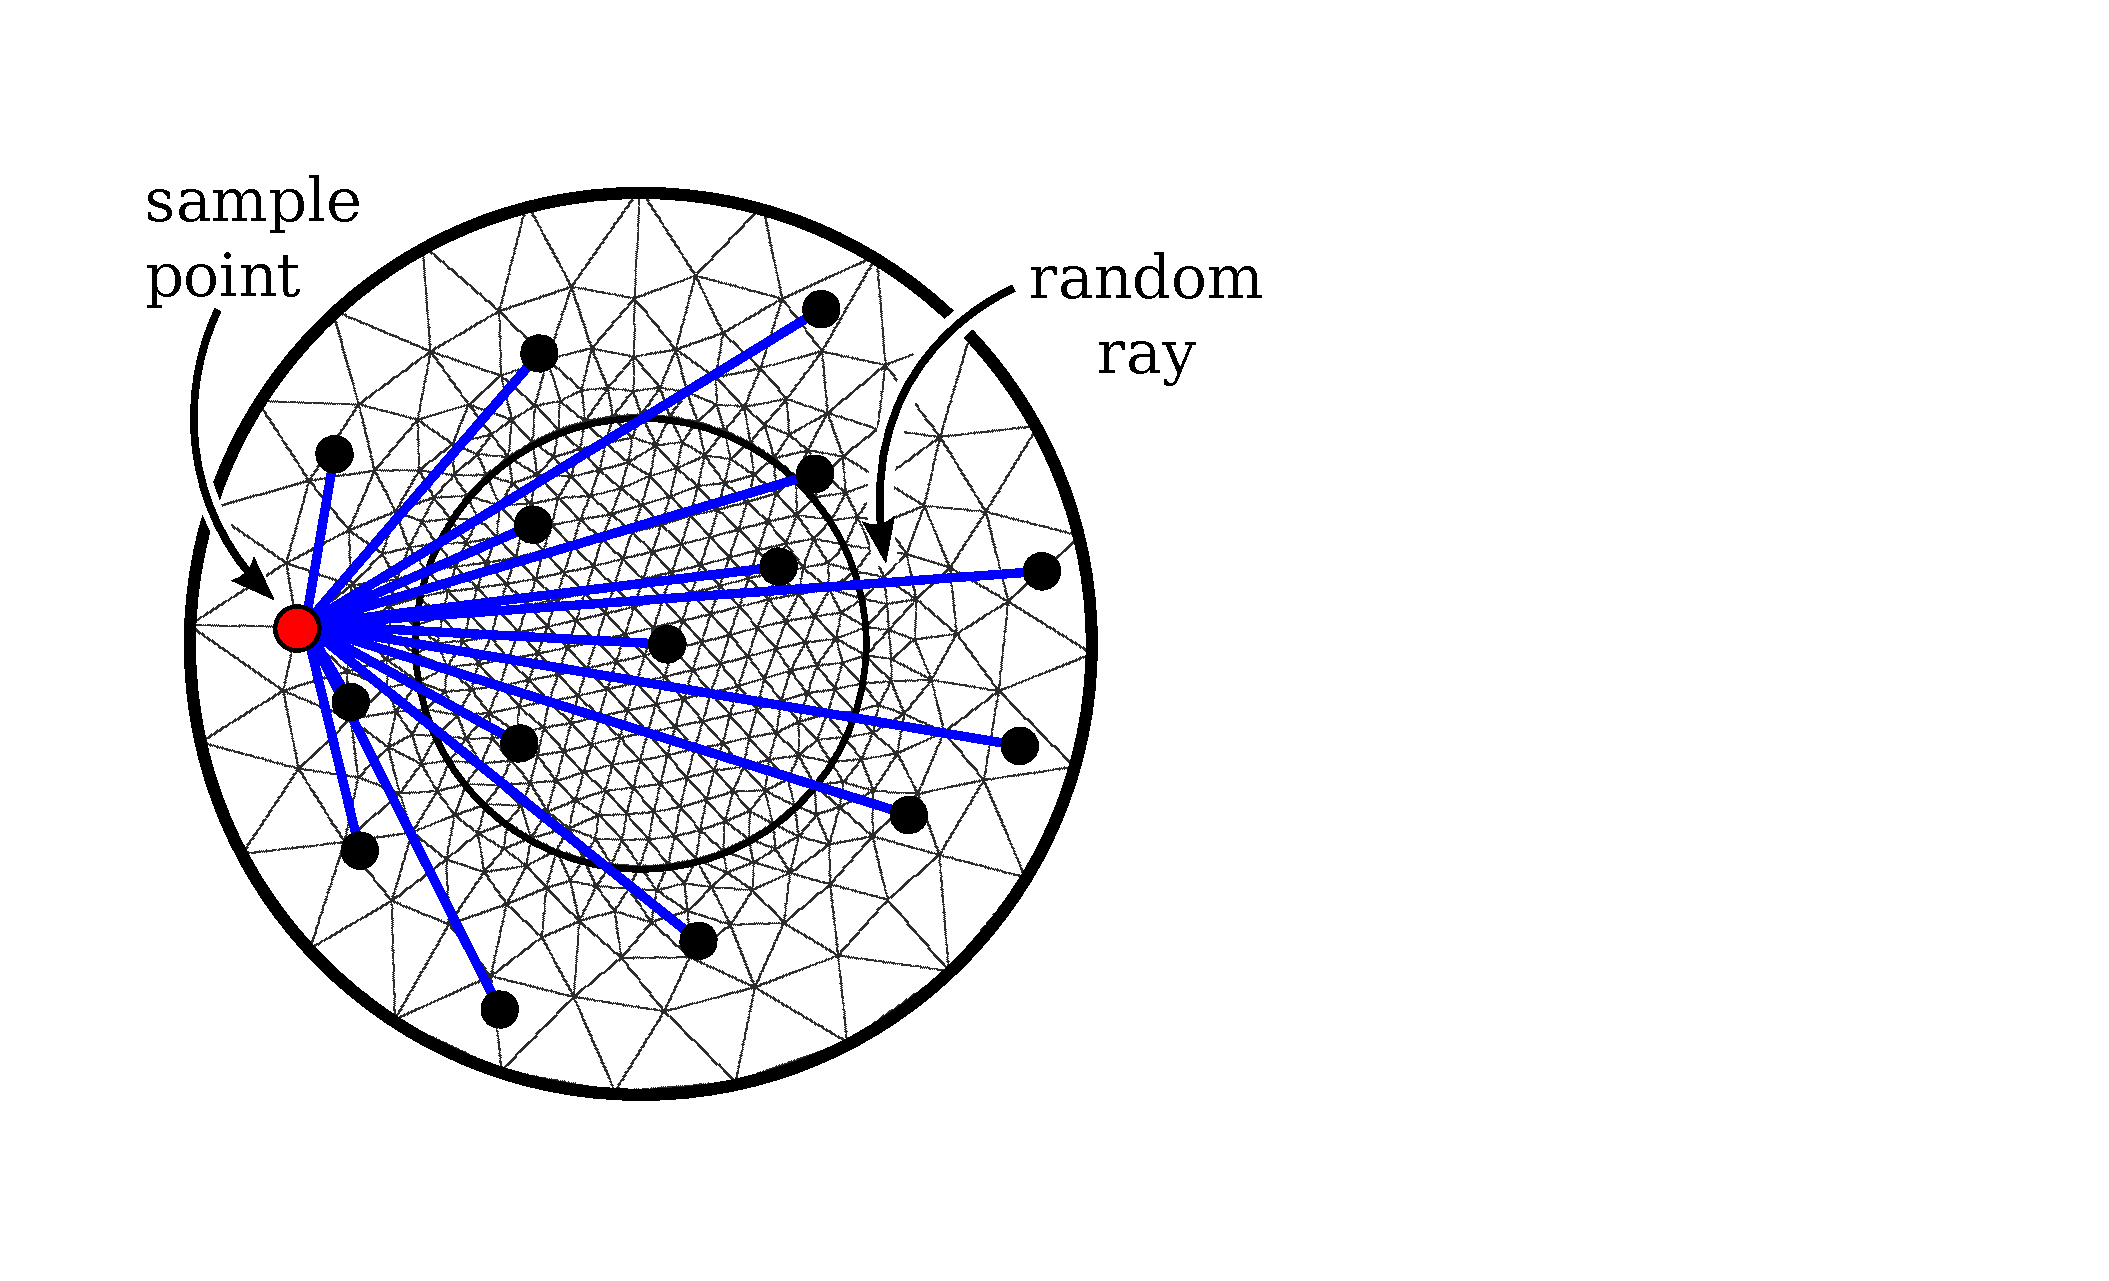
\includegraphics[height=0.55\paperheight]{graphics/monte_carlo_description_1.pdf}}
      \myonly{3}{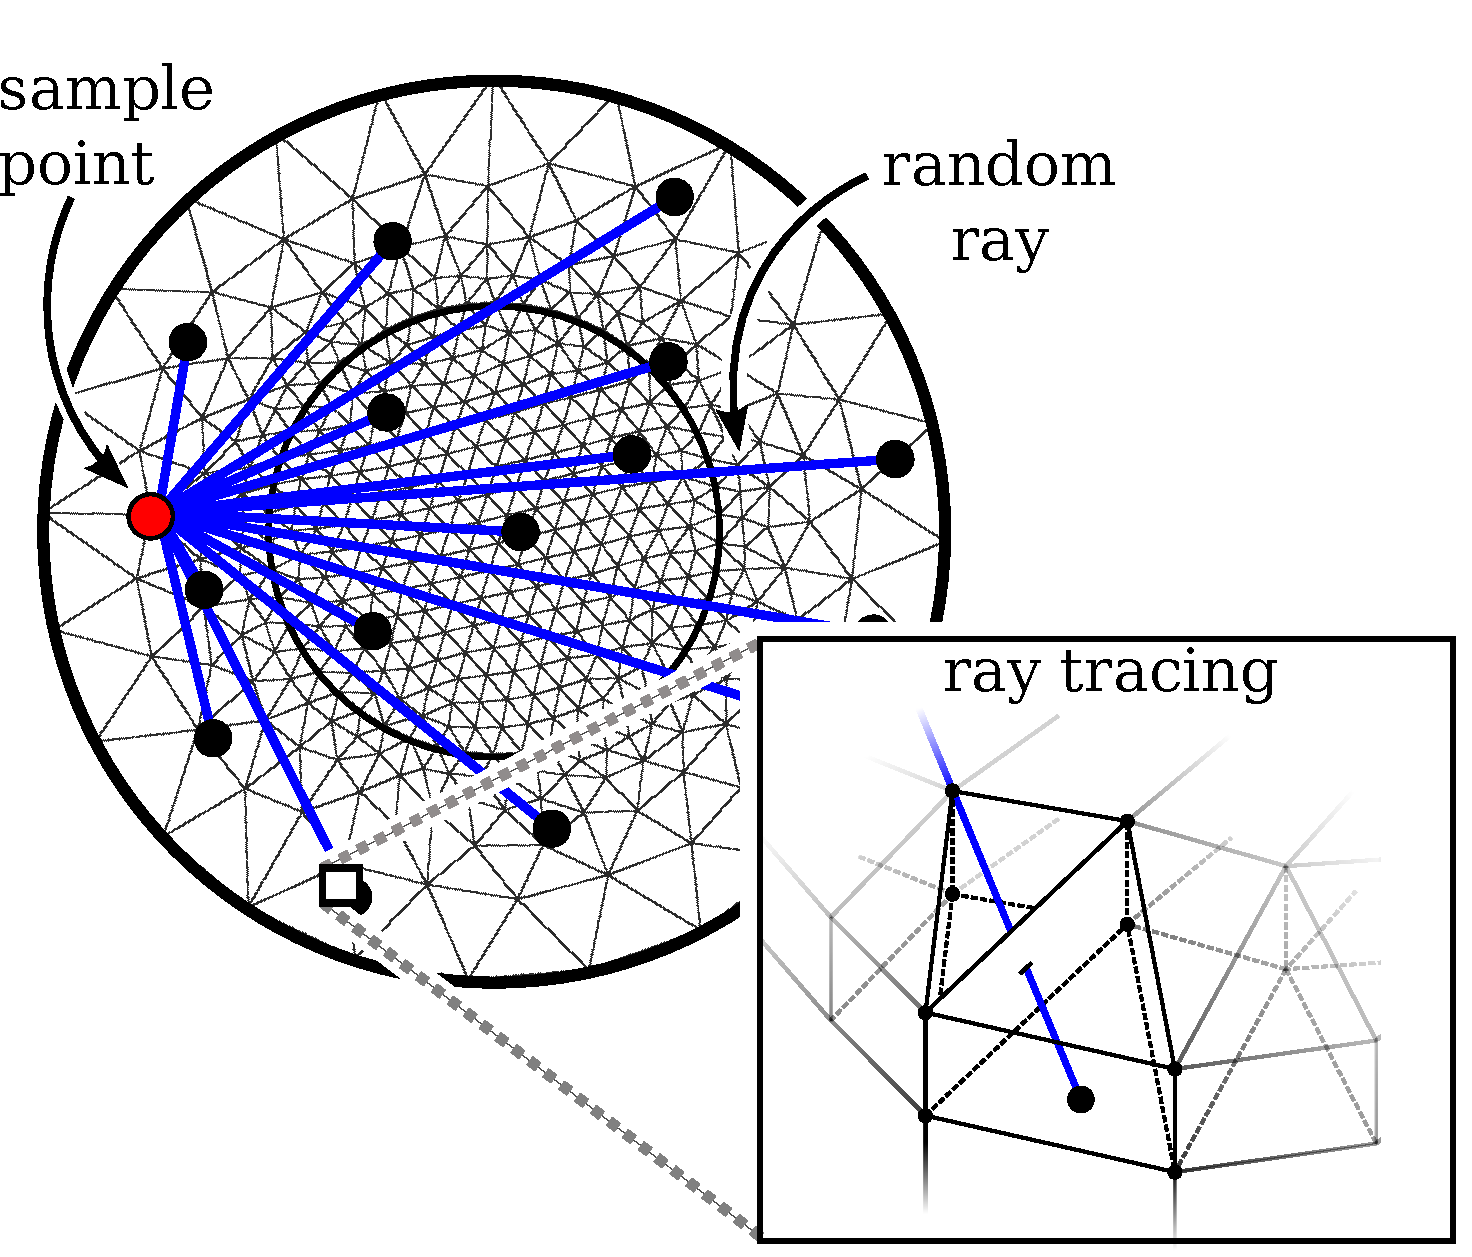
\includegraphics[height=0.55\paperheight]{graphics/monte_carlo_description_2.pdf}}
    \end{column}
    \begin{column}{.5\textwidth}
      \begin{itemize}
        \myuncover{1}{3}{
          \item Monte Carlo integration is one way to solve this integral
        }

        \myuncover{2}{3}{
          \item Create a statistical relevant amount of photons
        }
        \myuncover{3}{3}{
          \item Amplification of these photons can be simulated with ray tracing
        }
      \end{itemize}
    \end{column}
  \end{columns}
      \myonly{3}{\[ASE(sample~point)~=~\frac{1}{N}\sum_{i=1}^N amplification(photon_i)\]}
\end{frame}
